\chapter{Casi di studio e valutazioni}
In questa sezione verranno riportati i casi studio e i test effettuati sul framework. Tutti questi sono stati eseguiti su un sistema HPC Galielo-100 Cineca con le specifiche riportate nella tabella seguente

\vspace{.7cm}
\begin{center}
\begin{tabular}{l|l}
    \hline
    \textbf{Parameter} & \textbf{Value} \\
    \hline
    Number of nodes used & 3 \\
    \hline
    Processor & Intel CascadeLake 8260 \\
    \hline
    Number of sockets per node & 2 \\
    \hline
    Number of cores per socket & 24 \\
    \hline
    Memory size per node & 384 GB \\
    \hline
    Interconnect & Mellanox Infiniband 100GbE \\
    \hline
    OS & CentOS Linux \\ 
    \hline
    MPI & Open MPI  4.1.1 \\
    \hline
\end{tabular}
\label{table:hpc}
\end{center}

\section{Test}
Sono stati svolti diversi test al fine di trovare un modello ottimale di utilizzo e per la caratterizzazione di DDS, all'interno di sitemi HPC, nel contesto del Power Management. Nello specifico i test sono stati utili a capire il peso che avesse una singola configurazione o modello di utilizzo al fine di trovare quello più adeguato per una futura implementazione. I test effettuati sono:

\begin{itemize}
    \item test-1: protocollo di comunicazione
    \item test-2: partizioni e wildcards
    \item test-3: throughput
\end{itemize}


Al fine di condurli nel modo più trasparente e corretto possibile sono stati resi pubblici \cite{mygit} tutti i codici utilizzati durante lo svolgimento di questi test. %TODO5O: riordinare & documentare git

\subsection{Struttura dei test}
Sono stati prodotti dei test ad hoc, composti in parte da script bash, e in parte da programmi c++ con lo scopo di sfruttare al massimo le infrastruttura utilizzata \ref{table:hpc}. Ognuno di questi, con il fine di coprire e reperire il maggior numero di informazioni possibili, ha dovuto monitorare e catalogare 4 tipi di informazioni diversi:

\begin{itemize}
    \item Tempo solo invio
    \item Istruzioni Perf-Event
    \item Cicli TSC (read\_tsc)
    \item Tempo invio-ricezione
\end{itemize}
%TODO: se serve approfondire TSC, e metriche eseguite prima e dopo

In particolare nel Publisher \ref{actor:publisher} prima e dopo la chiamata a funzione di write() %TODO: inserire nella tesi?
si sono presi i valori tempo-invio, istruzioni, e TSC, mentre al lato ricevente, di Subscriber \ref{actor:subscriber} è stato preso il tempo al momento dell'arrivo del messaggio. Segue uno schema uml della base di ognuno dei test.
\begin{figure}[H]
    \centering
    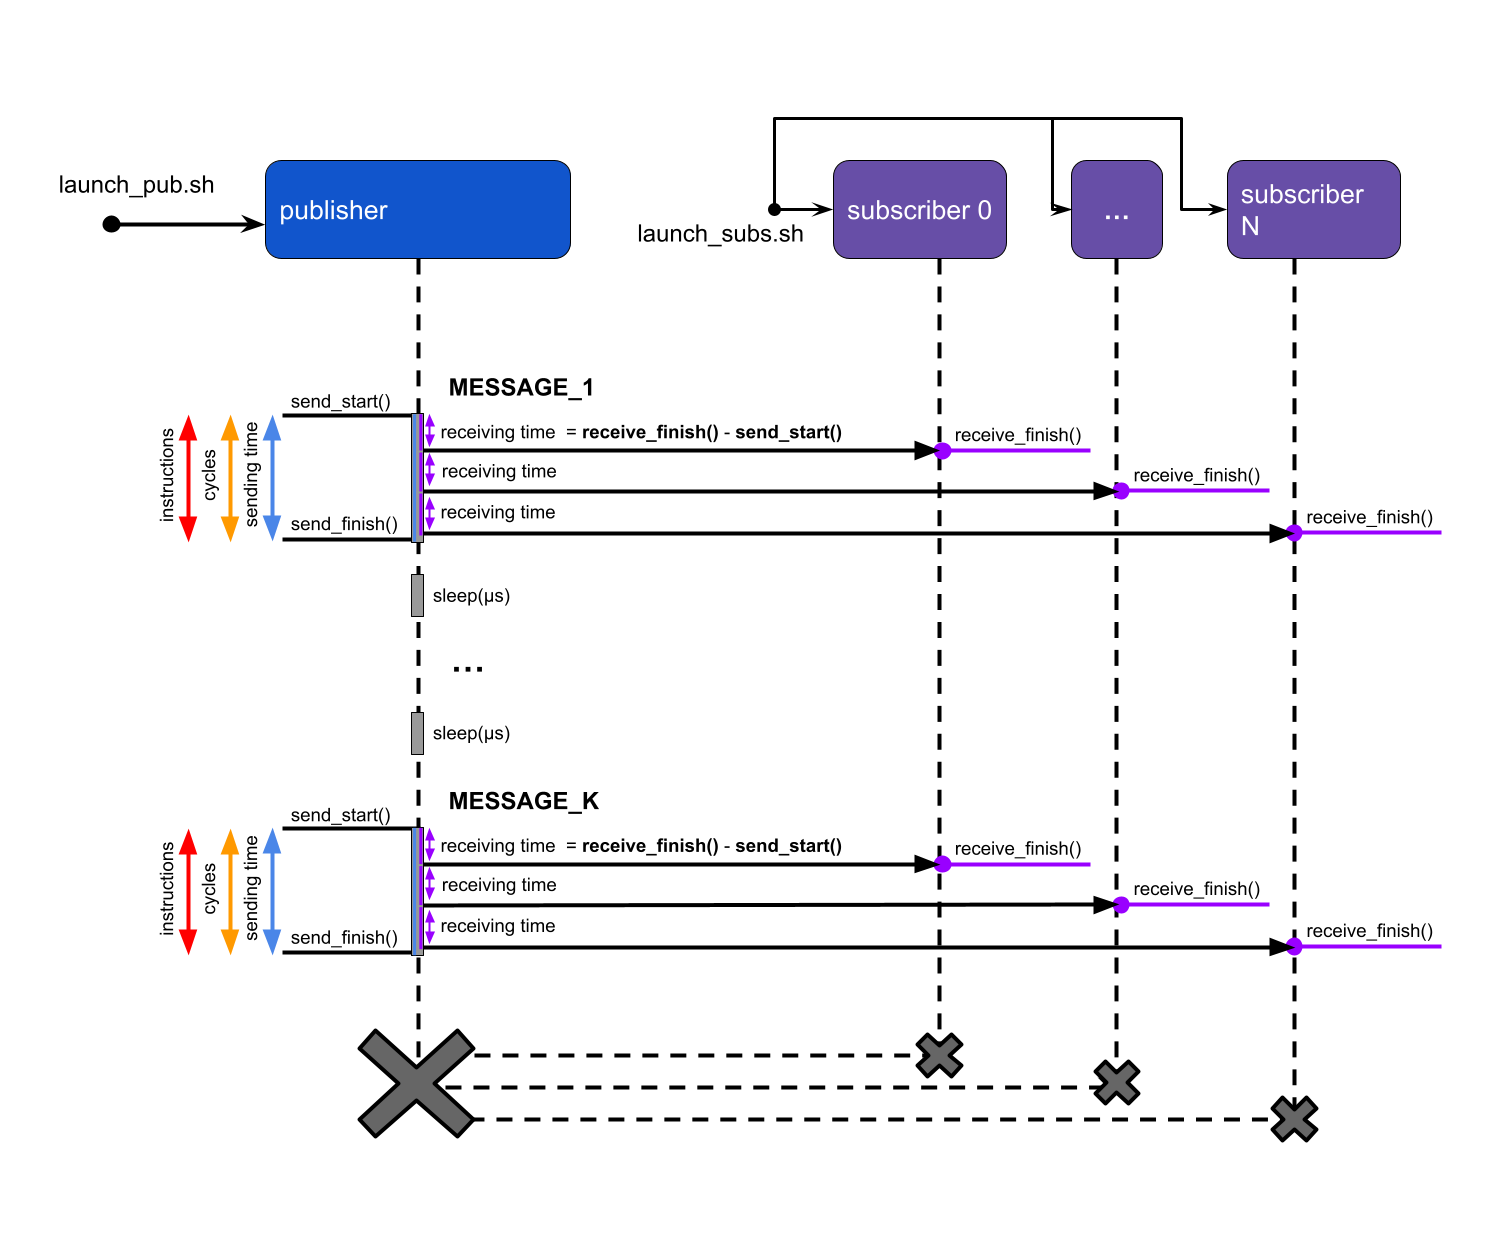
\includegraphics[width=\textwidth]{./img/umel-send-receive.png}
    \caption{Schema UML} %TODO: add readtsc, istr
    \label{fig:uml}
\end{figure}

\subsubsection{Sincronizzazione orologi su nodi diversi}
Per ottenere risultati attendibili sulla metrica del tempo è stato necessario sincronizzare i nodi utilizzati prima di poter far partire i test. Per farlo è stato usata una funzione \emph{CLOCK\_MONOTONIC} che rappresenta un \textit{un orologio non impostabile a livello di sistema che rappresenta il tempo monotono da un punto non specificato nel passato. Su Linux, quel punto corrisponde al numero di secondi di esecuzione del sistema da quando è stato avviato. L'orologio CLOCK\_MONOTONIC non è influenzato da salti discontinui nell'ora del sistema, ma è influenzato dalle regolazioni incrementali eseguite da  NTP.} Il problema che si è presentato, è che avendo nodi diversi su cui far eseguire i test, per provare ad esempio nel modo più affidabile i protocolli di trasporto, è stato necessario implementare delle MPI\_Barrier prima di diverse esecuzioni di \emph{clock\_gettime(CLOCK\_MONOTONIC)}. Di seguito sono stati riportati i grafici del risultato ottenuto.
\begin{figure}[H]
    \centering
    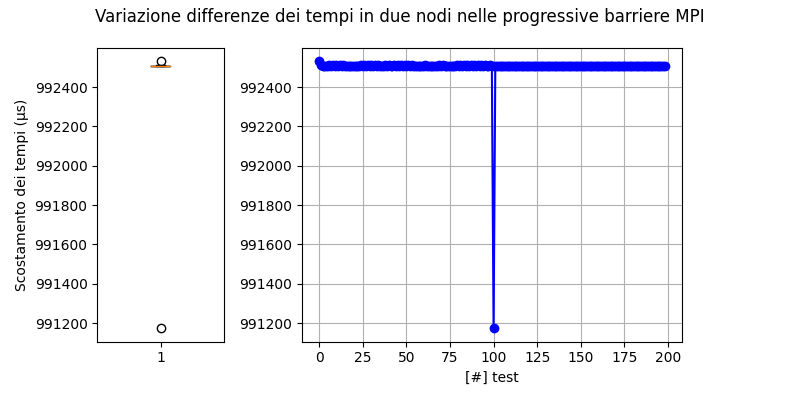
\includegraphics[width=\textwidth]{./results/time_sync_node.png}
    \caption{Scostamento del tempo su nodi diversi}
    \label{fig:sync_time_shift}
    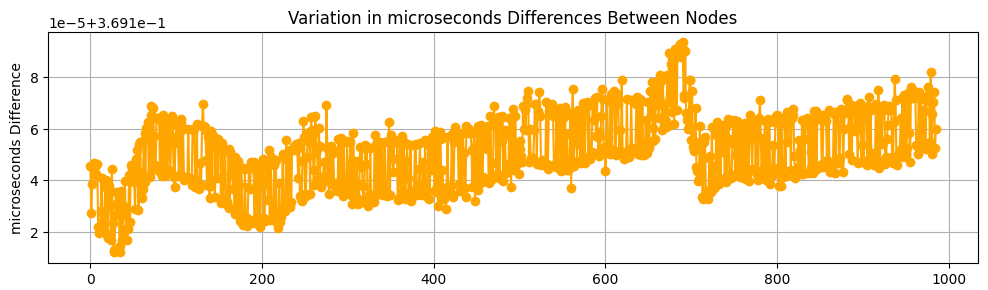
\includegraphics[width=0.99\textwidth]{./results/time_shift_clean.png}
    \caption{Scostamento senza outliers}
    \label{fig:sync_diff_distr}
    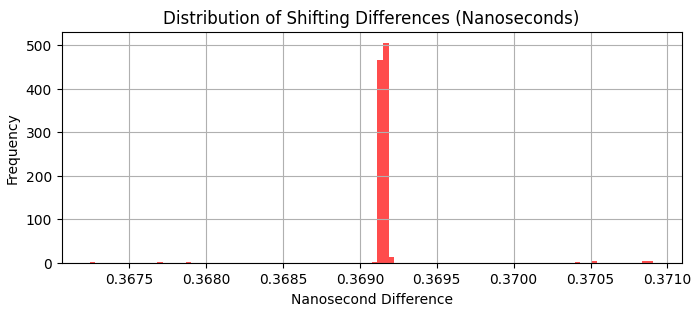
\includegraphics[width=\textwidth]{./results/time_sync_distribution.png}
    \caption{Distribuzione delle differenze}
    \label{fig:sync_diff_distr}
\end{figure}

Come possibile vedere nella figura \ref{fig:sync_time_shift} nonostante le mpi\_barrier, sono presenti degli scostamenti di tempo tra 2 nodi durante diversi test effettuati (in particolare 1000), e si è scelto di utilizzare il valore modale di questa differenza,sulla base del quale, si sono elaborati tutti i dati successivi.

\subsection{Impatto del numero di sub in un dominio}
Visto lo schema \ref{fig:uml} risulta facile capire, che il numero di subscriber presenti in un dominio comporta un overhead di comunicazione che va ad influenzare sia i tempi, che i cicli, che le istruzioni impiegate nella singola \emph{publish} su un topic che viene facilmente dimostrato nella figura\ref{fig:test3_overhead}.
\begin{figure}[H]
    \centering
    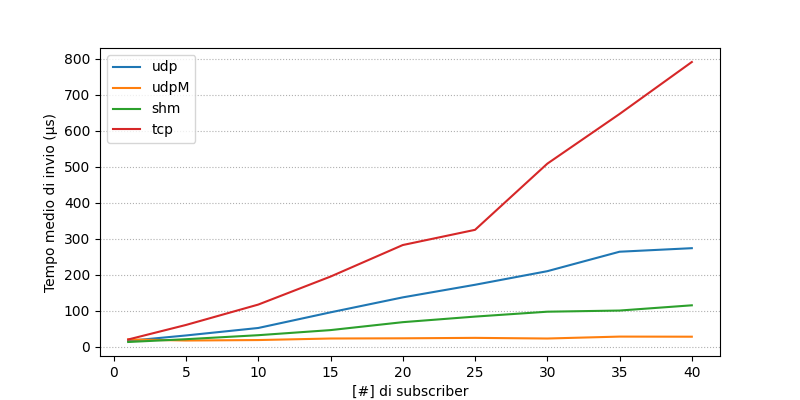
\includegraphics[width=\textwidth]{./results/test3_sending_multiplesub.png} %TODO, sqeunce is an error
    \caption{overhead sulla publish all'aumentare dei subscriber}
    \label{fig:test3_overhead}
\end{figure}
Ovviamente l'impatto è poco significativo in quei protocolli che applicano strutture di multicasting (spiegata successivamente) %TODO: aggiungere nel glossario
come udp-Multicast e Shared-Memory. 

\begin{figure}[H]
    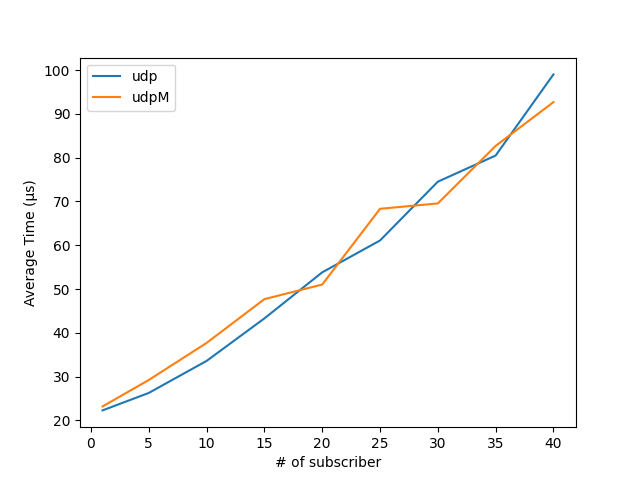
\includegraphics[width=\textwidth]{./results/test3_udpvsudpM.png} %TODO, sqeunce is an error
        \caption{}
        \label{}
\end{figure}

Questo può portare una singola publish a impiegare più cicli e più tempo della singola ricezione dei messaggi, come si vede nella figura\ref{fig:test3_different_protocols}

In tutti i test successivi, ove non specificato diversamente sono stati usati 1 publisher e 48 subscriber su diversi nodi. Questo è stato fatto per provare la scalabilità, visto che nel testbed che è stato utilizzato, erano presenti 48 core (1 core per ogni subscriber).

\subsection{Test-1}
In DDS ed in particolare nel layer sottostante di RTPS, per scambiare messaggi anche tramite rete, e non solo nello stesso nodo, è possibile scegliere come mezzo diversi tipi di protocolli:

\begin{itemize}
    \item udp: fornisce due versioni v4 e v6 e importa l'omonimo protocollo di trasporto
    \item tcp: fornisce due versioni v4 e v6 e importa l'omonimo protocollo di trasporto
    \item udp-multicast: una versione modificata del semplice udp, dove tutti i subscriber collegati allo stesso topic, hanno un indirizzo comune di ricezione dei dati, permettendo così al publisher di inviare un singolo messaggio che viene condiviso tra tutti i subscriber  % TODO: uml
    \item shared-memory: analogo al metodo precedentemente, ma invece di utilizzare un indirizzo IP, viene utilizzato un indirizzo di memoria. E' possibile solo quando i due processi che comunicano sono sullo stesso nodo, con memoria condivisa.
\end{itemize}

Nel primo test si è valutata la differenza di queste implementazioni utilizzando la rete infiniband \ref{table:hpc} su diversi nodi di un supercalcolatore. I risultati che sono stati trovati forniscono importanti informazioni, %TODO: to finish

\begin{figure}[H]
    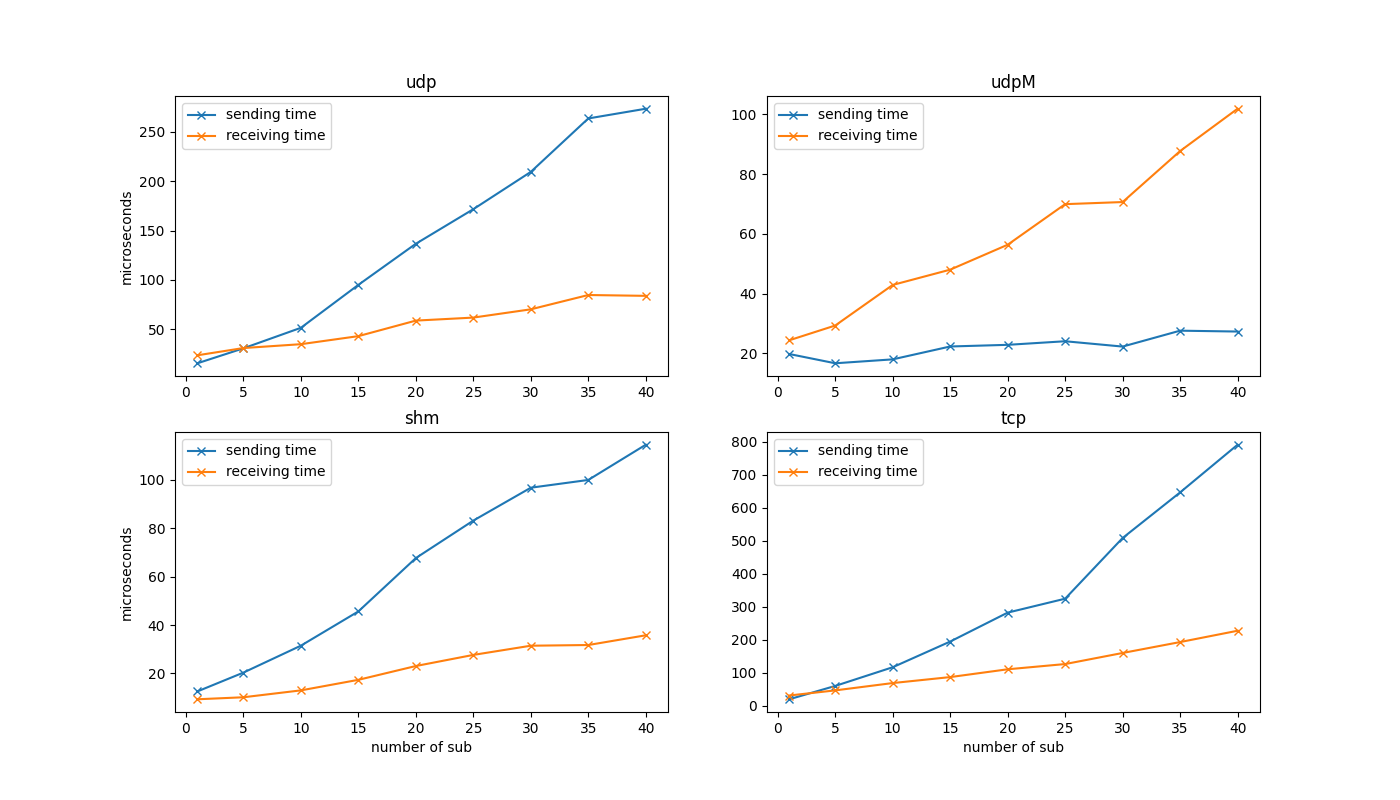
\includegraphics[width=\textwidth]{./results/test3_different_protocol_send_receive.png} %TODO, sqeunce is an error
        \caption{differenza tra solo publish e publish-subscribe per ogni protocollo}
        \label{fig:test3_different_protocols}
\end{figure}

\subsection{Test-2}
Un concetto fondamentale nelle comunicazioni tra attori con gerarchie diverse, in sistemi con diverse centinaia di migliaia di entita, come cluster, nodi, processori, workflow, job (etc.), sono le possibilità di instradare, segmentare e rendere gerarchiche le comunicazioni. Come spiegatolo nel capitolo \ref{Chapter:dds} in DDS ci sono diversi strumenti disponibili per farlo. Tra di loro differiscono per alcuni aspetti, come flessibilità, costo (in performance) e livello di segmentazione.

In questo test si è valutata la differenza in termini di performance dei diversi strumenti, con un particolare focus sulle partizioni e le wildcards rese disponibili in esso.

\subsubsection{Comparazione strumenti}
Nei test effettuati con domini, topic e partizioni, non sono state notate differenze degne di nota in termini di performance (cicli e istruzioni) nell'usare uno strumento piuttosto che un altro. 

\subsubsection*{Dominio} 
Il dominio è la segmentazione di più "forte" e di più alto livello. Va a partizionare gli attori presenti in un dominio in modo del tutto fisico (cambiando per ogni dominio porte e indirizzi di comunicazione) e per nulla flessibile. Per cambiare il dominio è necessario distruggere e creare di nuovo il partecipante. Inoltre il dominio non permette nessun tipo di gerarchia.
    
\subsubsection*{Topic}
All'interno di un dominio i topic definiscono il metodo principale di instradamento dei messaggi, essendo però limitato dal tipo di messaggio che si vuole inviare. Infatti topic diversi supportano tipi di dato diversi, e non sono modificabili a run-time. %TODO: glossario
Inoltre il topic non permette gerarchie ed è difficilmente modificabile a run-time

\subsubsection*{Partizione}
Questo strumento risulta molto interessante, in quanto all'interno di un topic permette di definire gerarchie (è possibile sottoscriversi a più partizioni contemporaneamente), definisce wildcards e crea una segmentazione virtuale. Inoltre è facilmente modificabile a run-time.

\subsubsection{Wildcards}
Le wildcards sono un costrutto appartenente alle partizioni, che permette di definire dei pattern testuali sulla base del quale vengono instradati i messaggi. Un esempio può essere \textit{Node*} che va a corrisponde a tutti i messaggi sotto il topic precedentemente definito, a tutte le partizioni che iniziano con Node.

\begin{figure}[H]
    \centering
    %TODO DA INSERIRE WILDCARDS costi
    %\includegraphics[width=\textwidth]{./results/}
\end{figure}


\subsection{Test-3}

\section{Risultati}

\section{Modello}

\section{Scheletro componenti}
Nel seguente capitolo viene stilato uno scheletro dei componenti con i relativi topic usati al fine di dare una visione completa e aggiuntiva rispetto al modello precedentemente stilato  
\begin{figure}[H]
    \centering
    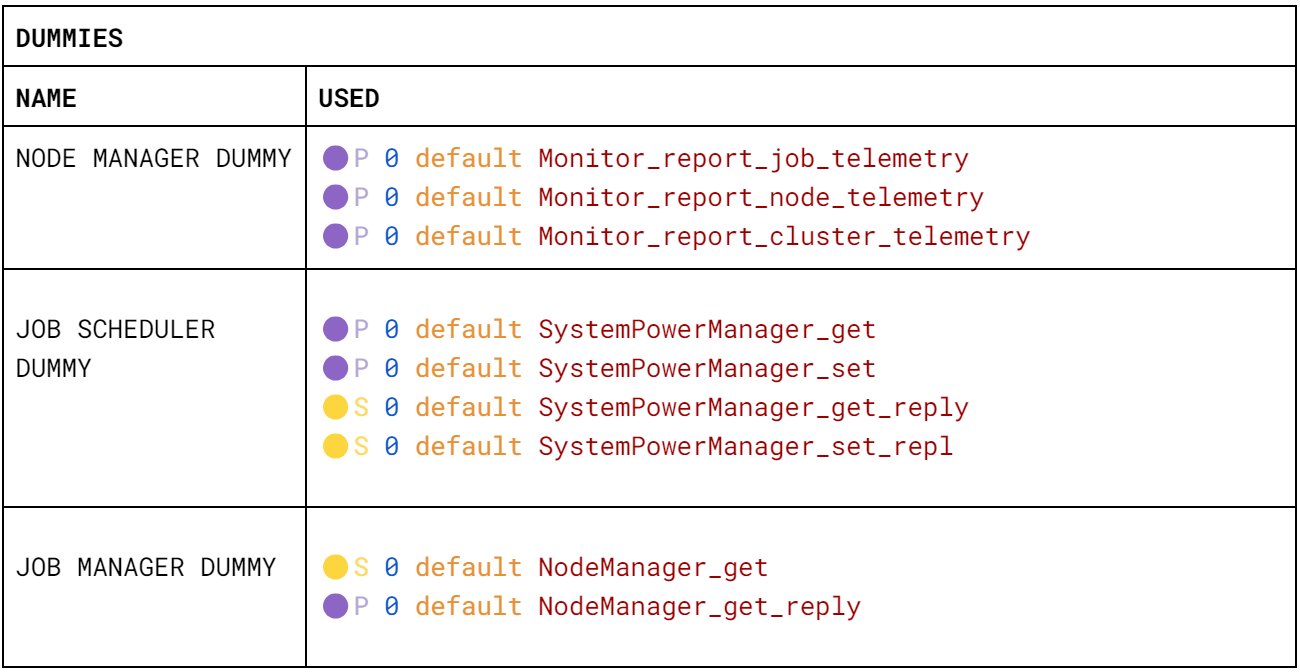
\includegraphics[width=\textwidth]{./img/dummies_skeleton.png}
    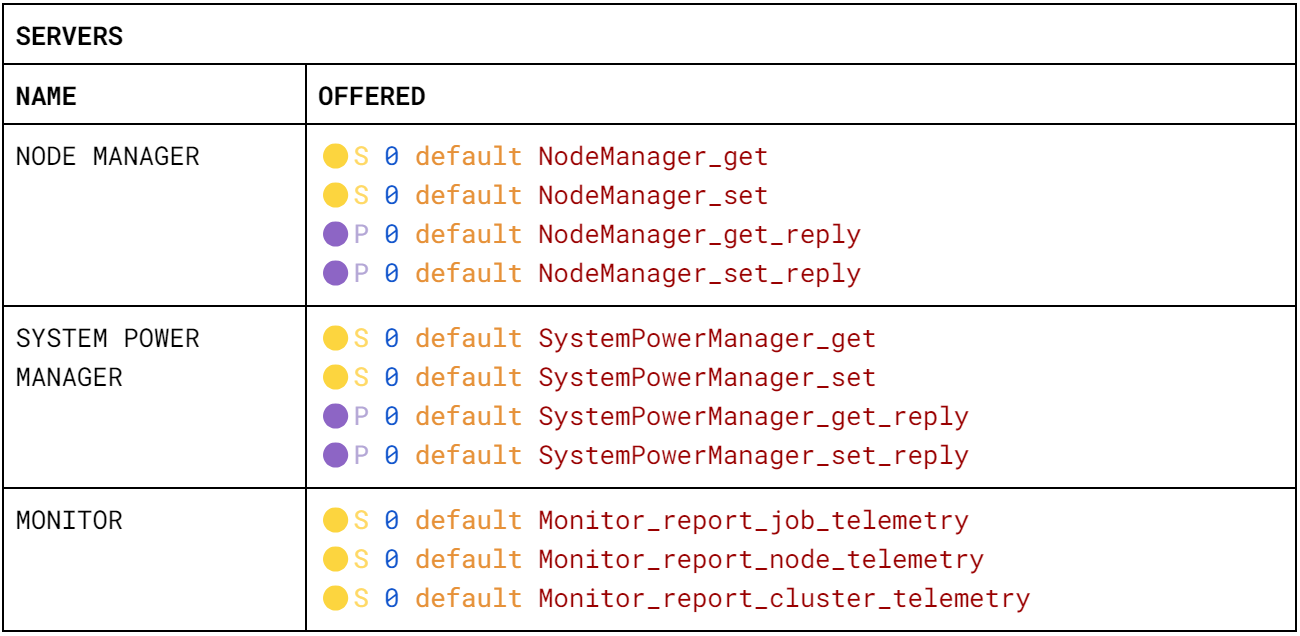
\includegraphics[width=\textwidth]{./img/server_skeleton.png}
\end{figure}
